%%%%%%%%%%%%%%%%%%%%%%%%%%%%%%%%%%%%%%%%%%%%%%%%%%%%%%%%%%%%%%%%%%%%%%%%
%                                                                      %
%     File: Current_Reference.tex                                      %
%     Tex Master: Thesis.tex                                           %
%                                                                      %
%     Author: Israel Sother                                            %
%     Last modified: 27 May 2024                                       %
%                                                                      %
%%%%%%%%%%%%%%%%%%%%%%%%%%%%%%%%%%%%%%%%%%%%%%%%%%%%%%%%%%%%%%%%%%%%%%%%
\section{Current References}
\label{section:Current_references}
\vfill

To simplify the real-time computations, the current references can be calculated offline. A simple approach would be to only consider the quadrature current $i_q$ as the main component of torque, and compute the reference using the torque constant. This approach is simple and fast, but it does not account for the motor's inductance, which can be used to increase efficiency. The maximum torque per ampere strategy actively uses the inductance differences between the direct and quadrature axes to get the maximum torque for a given current, but as the inductances are variable, the optimal current reference is also variable. This section aims to calculate the optimal references for the current at all operating points and generate a lookup table for the real-time controller.

Although it is possible to use the \gls{mpc} to optimize the current references, doing it offline not only allows for faster computational times but also results in more precise references. The downside of this approach is that it negates the possibility of acting upon online parameter estimation, however, this drawback can be mitigated by implementing regular calibration procedures.

As efficiency is one of the objectives, a good approach is to maximize the torque generated by a given current $i = \sqrt{i_d^2 + i_q^2}$. This strategy is called \gls{mtpa}, and when there aren't constraints it becomes a simple problem defined in \Cref{eq:mtpa_problem}.
\begin{equation}
	\begin{aligned}
		\max_{i_d,i_q} \quad & p\, i_q((L_d - L_q)i_d + \psi_{PM}) \\
		\rm{s.t.}  \quad & i = \sqrt{i_q^2 + i_d^2}            \\
	\end{aligned}
	\label{eq:mtpa_problem}
\end{equation}
To optimize~\ref{eq:mtpa_problem}, one can write the problem using Lagrange multipliers ($\lambda$), as in \Cref{eq:mtpa_lagrange}.
\begin{equation}
	\mathcal{L} = p\, i_q((L_d - L_q)i_d + \psi_{PM}) - \lambda(\sqrt{i_q^2 + i_d^2} - i)
	\label{eq:mtpa_lagrange}
\end{equation}
The partial derivatives of the Lagrange function are defined in \Cref{eq:mtpa_lagrange_partial}.
\begin{subequations}
	\begin{equation}
		\frac{\partial \mathcal{L}}{\partial i_d}  = p\,i_q(L_d - L_q) - \frac{\lambda i_d}{\sqrt{i_d^2 + i_q^2}}
		\label{eq:lagrange_partial1}
	\end{equation}
	\begin{equation}
		\frac{\partial \mathcal{L}}{\partial i_q}  = p((L_d - L_q)i_d + \psi_{PM}) - \frac{\lambda i_q}{\sqrt{i_d^2 + i_q^2}}
		\label{eq:lagrange_partial2}
	\end{equation}
	\begin{equation}
		\frac{\partial \mathcal{L}}{\partial \lambda}  = \sqrt{i_q^2 + i_d^2} - i
		\label{eq:lagrange_partial3}
	\end{equation}
	\label{eq:mtpa_lagrange_partial}
\end{subequations}
Now, equating the partial derivatives to zero, and replacing \Cref{eq:lagrange_partial1} in \Cref{eq:lagrange_partial2} and \Cref{eq:lagrange_partial3} yields \Cref{eq:lagrange_partial20}.

\begin{subequations}
	\begin{equation}
		i = \sqrt{i_q^2 + i_d^2}
		\label{eq:lagrange_partial21}
	\end{equation}
	\begin{equation}
		\frac{\lambda i_d}{i}  = p\,i_q(L_d - L_q)
		\label{eq:lagrange_partial22}
	\end{equation}
	\begin{equation}
		\frac{\lambda i_q}{i}  = p((L_d - L_q)i_d + \psi_{PM})
		\label{eq:lagrange_partial23}
	\end{equation}
	\label{eq:lagrange_partial20}
\end{subequations}
Isolating $\lambda$ in \Cref{eq:lagrange_partial23} and replacing it on  \Cref{eq:lagrange_partial22}, results in \Cref{eq:mpta_intermediary}.

% \begin{subequations}
% \begin{equation}
% 	\frac{\lambda i_d}{i}  = p\,i_q(L_d - L_q)
% \end{equation}
% \begin{equation}
% 	\lambda   = \frac{i}{i_q}p((L_d - L_q)i_d + \psi_{PM})
% \end{equation}
% \end{subequations}
% \\
\begin{equation}
	\frac{p((L_d - L_q)i_d + \psi_{PM}) i_d}{i_q}  = p\,i_q(L_d - L_q)
	\label{eq:mpta_intermediary}
\end{equation}
Rearranging to a quadratic form produces \Cref{eq:mpta_intermediary2}.

% \begin{equation}
% 	((L_d - L_q)i_d + \psi_{PM}) i_d  = i_q^2(L_d - L_q)
% \end{equation}
% \\
% \begin{equation}
% 	(L_d - L_q)i_d^2 + i_d\psi_{PM}   = i_q^2(L_d - L_q)
% \end{equation}
% \\
% \begin{equation}
% 	i_d\psi_{PM}   = (i_q^2-i_d^2)(L_d - L_q)
% \end{equation}
% \\
% \begin{equation}
% 	\frac{i_d}{i_q^2-i_d^2} = \frac{L_d - L_q}{\psi_{PM}}
% 	\label{eq:mtpa_ref}
% \end{equation}
% \\
% \begin{equation}
% 	i_d = (i_q^2-i_d^2)\frac{L_d - L_q}{\psi_{PM}}
% \end{equation}
% \\
\begin{equation}
	i_d+i_d^2\frac{L_d - L_q}{\psi_{PM}} = i_q^2\frac{L_d - L_q}{\psi_{PM}}
	\label{eq:mpta_intermediary2}
\end{equation}
Solving for $i_d$ results in \Cref{eq:mpta_intermediary3}.
\begin{equation}
	i_d = \pm\frac{\sqrt{4 {\left(\frac{L_d - L_q}{\psi_{PM}}\right)}^2 {i_q}^2 +1}-1}{2\frac{L_d - L_q}{\psi_{PM}}}
	\label{eq:mpta_intermediary3}
\end{equation}
But comparing with the torque equation is clear that the negative option would not maximize the torque, thus, the final result is \Cref{eq:mtpa_ref}.
\begin{equation}
	i_d = \frac{\sqrt{4 {\left(\frac{L_d - L_q}{\psi_{PM}}\right)}^2 {i_q}^2 +1}-1}{2\frac{L_d - L_q}{\psi_{PM}}}
	\label{eq:mtpa_ref}
\end{equation}

This equation is valid for a constant inductance and with no constraints. If the inductance curve is used then an iterative approach can solve the algebraic loop of the inductances. If the inductances are assumed to be monotonically decreasing, then the iterative approach is guaranteed to converge to the proper value, resulting in \Cref{fig:mtpa_simple}.

\begin{figure}[!htb]
	\centering
	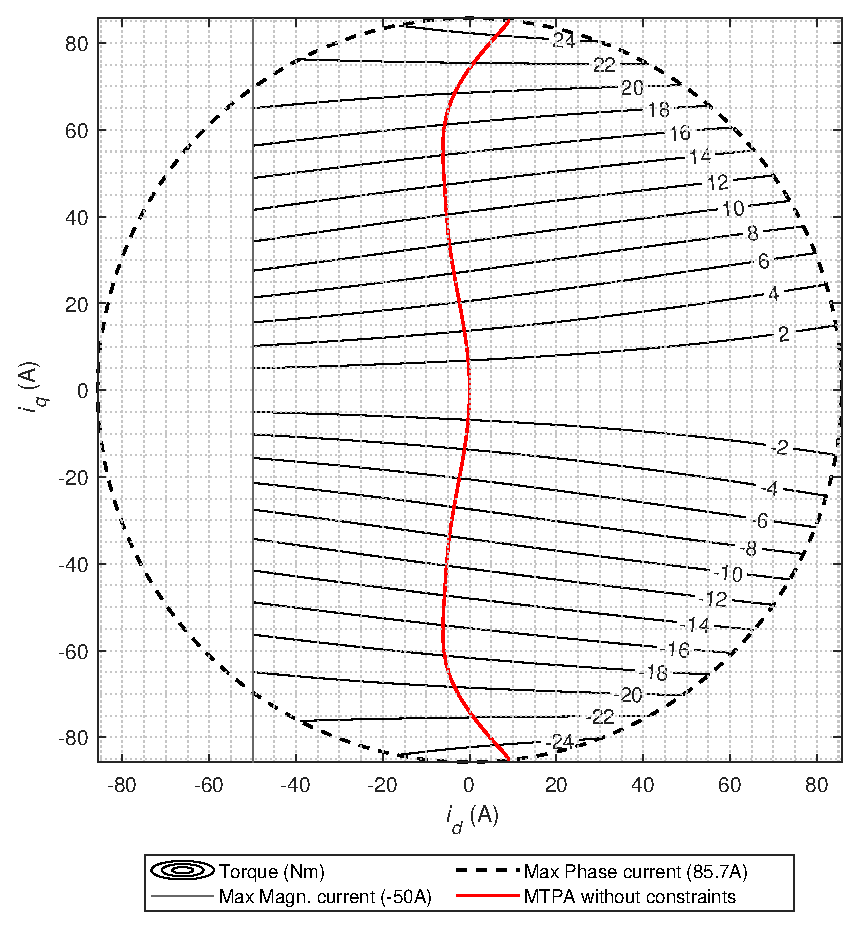
\includegraphics[width=0.6\textwidth]{Figures/Torque_MTPA_simple.eps}
	\caption[Maximum Torque per Ampere curve without constraints.]{Maximum Torque per Ampere curve without constraints.}
	\label{fig:mtpa_simple} %chktex 24
\end{figure}

\subsection{Constraints with limited input voltage}

While direct, the presented approach does not account for voltage limitations, meaning that when the rotor speed increases the back emf becomes large enough to limit the current operation points. To account for that the voltage constraint must be defined.

If the current is assumed to be constant, \Cref{eq:motor_with_inductances_no_derivative} can be rearranged to calculate the maximum current for a given voltage and velocity as in \Cref{eq:voltage_constraint_model}, with the voltage constraint defined in \Cref{eq:voltage_constraint_vdc}.
% \begin{subequations}
% 	\begin{equation}
% 		0 =u_d -r i_d +\omega_e L_q i_q
% 	\end{equation}
% 	\begin{equation}
% 		0 = u_q -r i_q - \omega_e (L_d i_d +\psi_{PM})
% 	\end{equation}
% \end{subequations}

\begin{subequations}
	\begin{equation}
		u_d = r i_d -\omega_e L_q i_q
	\end{equation}
	\begin{equation}
		u_q =  r i_q + \omega_e (L_d i_d +\psi_{PM})
	\end{equation}
    \label{eq:voltage_constraint_model} %chktex 24
\end{subequations}
\begin{equation}
	\sqrt{u_d^2+u_q^2}\leq V_{DC}
    \label{eq:voltage_constraint_vdc} %chktex 24
\end{equation}

Subjecting \Cref{eq:voltage_constraint_model} to \Cref{eq:voltage_constraint_vdc} an ellipse equation is obtained, where the center is defined by the rotor speed and the flux linkage, while the radius is defined by the DC link voltage and the resistance. The ellipse is defined as in \Cref{eq:voltage_ellipse}.
% \begin{equation}
% 	\psi_d = L_di_d + \psi_{PM}
% \end{equation}
% \begin{equation}
% 	\psi_q = L_qi_q
% \end{equation}

\begin{equation}
	{(r i_d -\omega_e \psi_q)}^2 + {(r i_q + \omega_e \psi^*_d)}^2\leq V_{DC}^2
	\label{eq:voltage_ellipse} %chktex 24
\end{equation}

Here $\psi^*_d = L_d i_d + \psi_{PM}$ and $\psi_q = L_q i_q$. Note that this ellipse size dynamically changes depending on the instantaneous rotor velocity and DC link voltage.

Using the ellipse as a constraint, \Cref{eq:mtpa_problem} can be rewritten as in \Cref{eq:mtpa_problem_with_voltage_constraint}, where the speed and DC link voltage are known.
This optimization problem tries to minimize the current modulus, while matching the produced torque with the reference torque and keeping the currents inside the voltage elipse constraint.
\begin{equation}
	\begin{aligned}
		\min_{i_d,i_q} \quad & \sqrt{i_q^2 + i_d^2} \\
		\rm{s.t.}  \quad & T_{ref} = p\, i_q((L_d - L_q)i_d + \psi_{PM})\\
		               \quad & {(r i_d -\omega_e \psi_q)}^2 + {(r i_q + \omega_e \psi^*_d)}^2\leq V_{DC}^2            \\
	\end{aligned}
	\label{eq:mtpa_problem_with_voltage_constraint} %chktex 24
\end{equation}

This optimization problem was formulated on \textit{MATLAB} for several speeds and voltages. Some of the main cases are shown in \Cref{fig:mtpa_constrained}. On this graph, the iso-torque lines show the current combinations that yield the same torque, independent of the velocity or the voltage. The voltage ellipses are defined from the rotor velocity and the current DC link voltage, and they assume that the current is constant. The area contained by the ellipse is the feasible region at that speed and supply voltage. Steady-state operation at any point outside the ellipse would require a speed reduction or a voltage increase.
% figures \ref{fig:mtpa_Constrained_420}, \ref{fig:mtpa_Constrained_540}, and \ref{fig:mtpa_Constrained_588}.
% \begin{figure}[H]
% 	\centering
% 	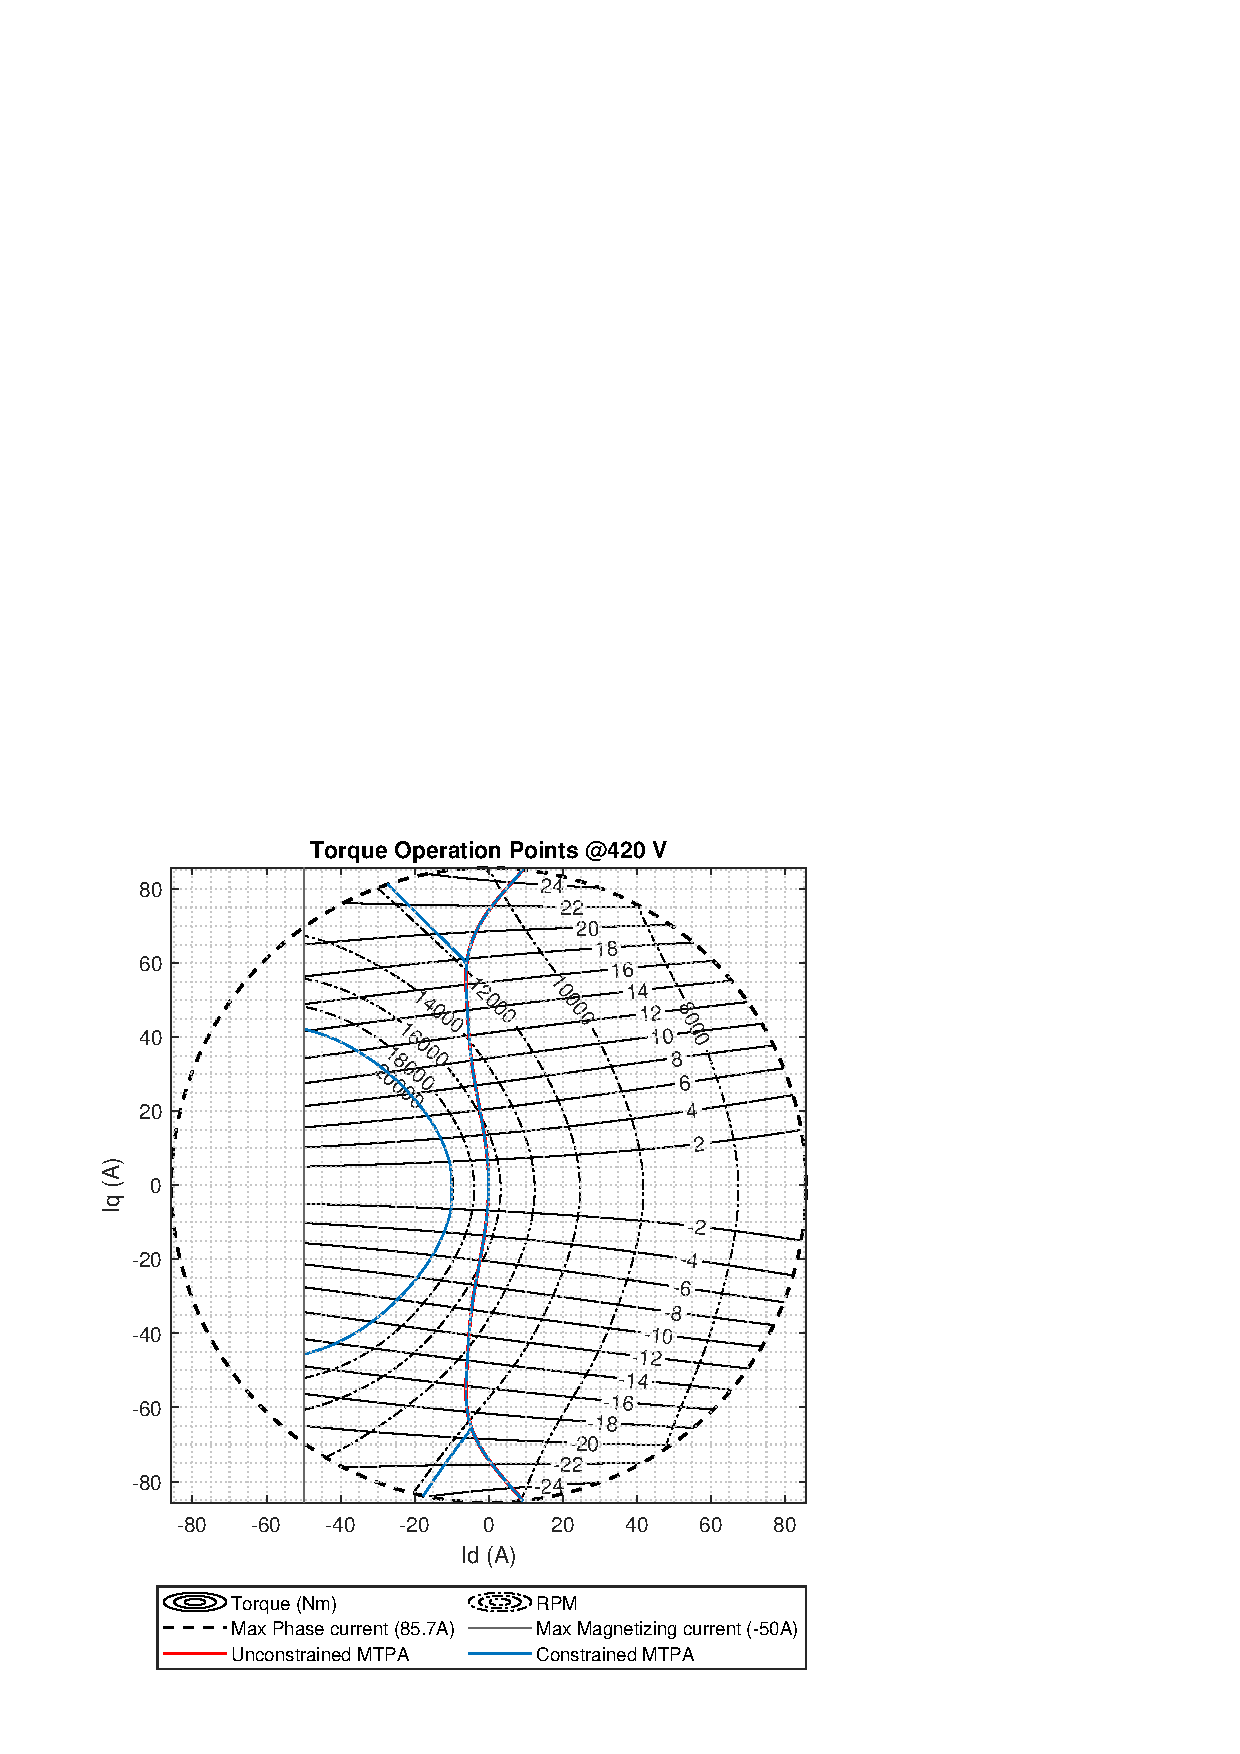
\includegraphics[width=0.65\textwidth]{Figures/Motor_map@420V.png}
% 	\caption[Maximum Torque per Ampere curve constrained @420V.]{Maximum Torque per Ampere curve constrained @420V}
% 	\label{fig:mtpa_Constrained_420} %chktex 24
% \end{figure}
% \begin{figure}[H]
% 	\centering
% 	\includegraphics[width=0.65\textwidth]{Figures/Motor_map@540V.png}
% 	\caption[Maximum Torque per Ampere curve constrained @540V.]{Maximum Torque per Ampere curve constrained @540V}
% 	\label{fig:mtpa_Constrained_540} %chktex 24
% \end{figure}
% \begin{figure}[H]
% 	\centering
% 	\includegraphics[width=0.65\textwidth]{Figures/Motor_map@588V.png}
% 	\caption[Maximum Torque per Ampere curve constrained @588V.]{Maximum Torque per Ampere curve constrained @588V}
% 	\label{fig:mtpa_Constrained_588} %chktex 24
% \end{figure}
\begin{figure}[!htb]
	\begin{subfigmatrix}{2}
		\subfigure[Minimum Voltage]{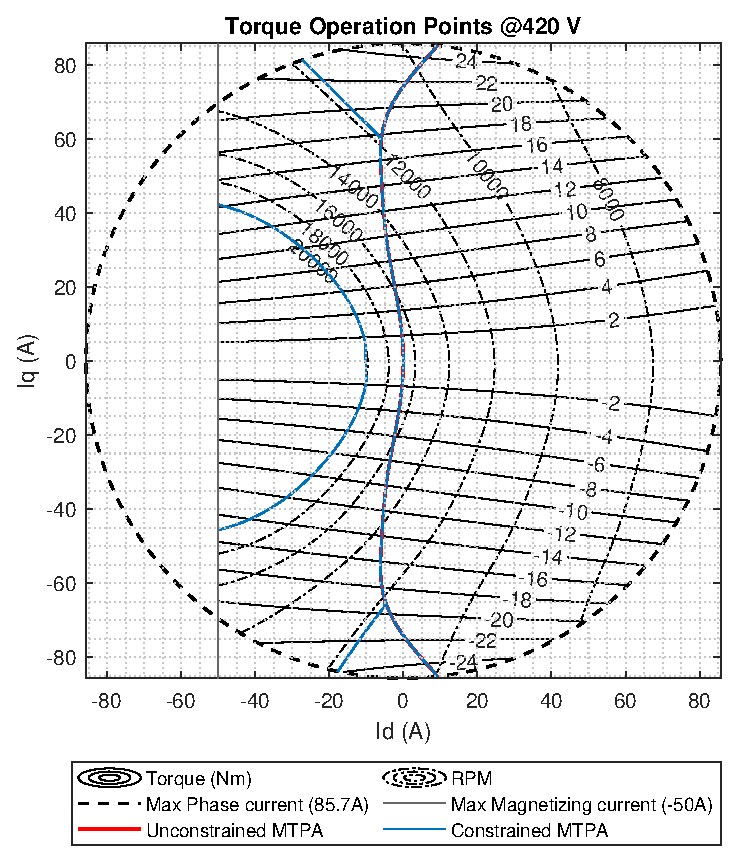
\includegraphics[width=0.49\linewidth]{Figures/Motor_map@420V}\label{fig:mtpa_Constrained_420}}
		\subfigure[Nominal Voltage]{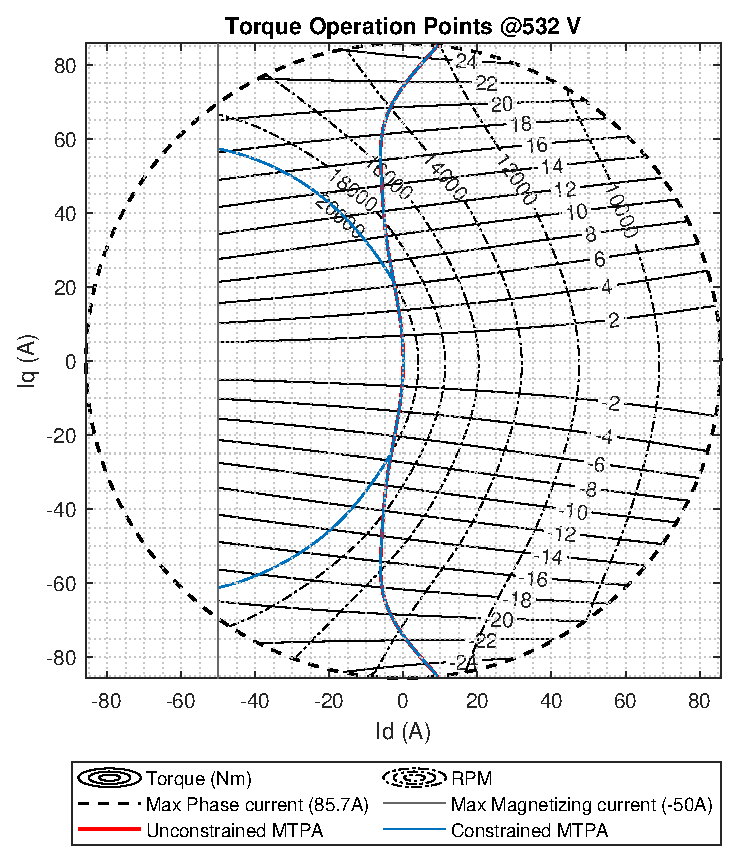
\includegraphics[width=0.49\linewidth]{Figures/Motor_map@532V}\label{fig:mtpa_Constrained_540}}
	\end{subfigmatrix}
	\begin{subfigmatrix}{1}
		\subfigure[Maximum Voltage]{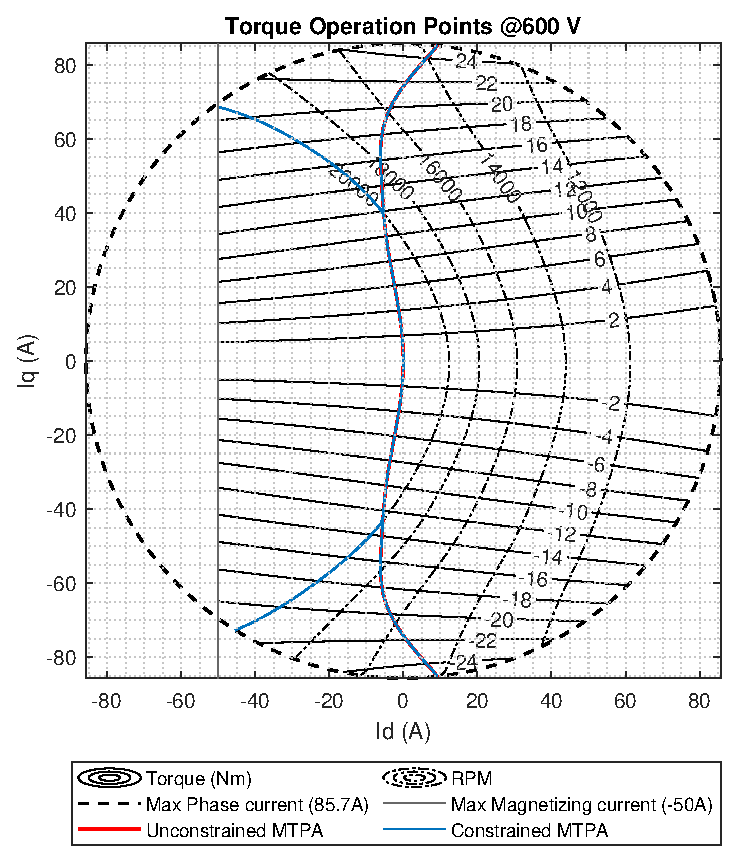
\includegraphics[width=0.49\linewidth]{Figures/Motor_map@600V}\label{fig:mtpa_Constrained_588}}
	\end{subfigmatrix}
	\caption{Constrained Maximum Torque per Ampere curve at minimum, nominal, and maximum voltages. Reference currents are shown for 0, 13000 and 2000 RPMs.}
	\label{fig:mtpa_constrained}%chktex 24
\end{figure}

Note that while the torque map is symmetrical relating to the $i_d$ axis, the voltage ellipse is not, it has been rotated slightly in an anti-clockwise direction. This rotation is due to the resistance of the phases that when the machine is working as a motor, reduce the total available voltage to fight the \gls{emf}.\@ If the phase resistance is low the ellipse becomes aligned with the $i_d$ axis. Another important remark is the center of the voltage ellipse, as the AMK motor has permanent magnets with strong flux linkage the ellipse center is shifted farther away from the origin, but in a reluctance machine, the center would be at the origin, the same as the torque. Special cases appear when the ellipse center is inside the feasible current region, as the voltage-limited speed goes to infinity. An important location in this graph is the motor characteristic point, which can be easily located as being the place where the maximum phase current circumference yields the higher torque. The speed at this point is the motor's characteristic speed, and if the graph is created for the motor's nominal voltage, that becomes also the nominal speed of the motor. This point is important as any further increase in speed will result in a reduction in the maximum motor torque.

Figure~\ref{fig:mtpa_constrained} clearly shows that the optimal current reference is the \gls{mtpa} while the velocity and voltages allow it, and after that, the voltage ellipse becomes the best alternative. It is important to understand that the voltage constraint is dependent on the combination of DC Link voltage and rotor speed, when the voltage increases the ellipse for a given speed expands, allowing further operation on the unconstrained \gls{mtpa} line. This not only increases efficiency (as it produces the same torque with less current) but also improves performance, pushing the motor characteristic point further on the torque vs rpm diagram. 

Some processing is still needed to account for points outside of the feasible region, but the presented graphs can be used as a motor map,  where given the current DC Link voltage, motor speed, and desired torque, it returns the reference currents to optimally reach the torque reference. This can also be expanded to include temperature effects. 

\subsection{Inductance Curves}
\label{section:inductance_curves_current_reference}

The inductance curves used to generate the motor maps presented in \Cref{section:Current_references} were obtained from a spreadsheet provided by the manufacturer that contained simulation data. The inductances computed from it are presented in \Cref{fig:inductance_manufacturer}. However, for the sake of completeness, the current reference curves generated from the inductance values obtained through characterization (\Cref{fig:inductances_method_2}) are included in the \Cref{chapter:appendix_current_reference}. This was necessary because a working testbench with stable control was needed to properly characterize the inductances. This characterization was completed after the implementation of the control in the experimental setup. Unfortunately, shortly after, testbench limitations impeded further testing. Consequently, the maps generated using the characterization inductance curves were not tested experimentally.

\begin{figure}[!htb]
	\centering
	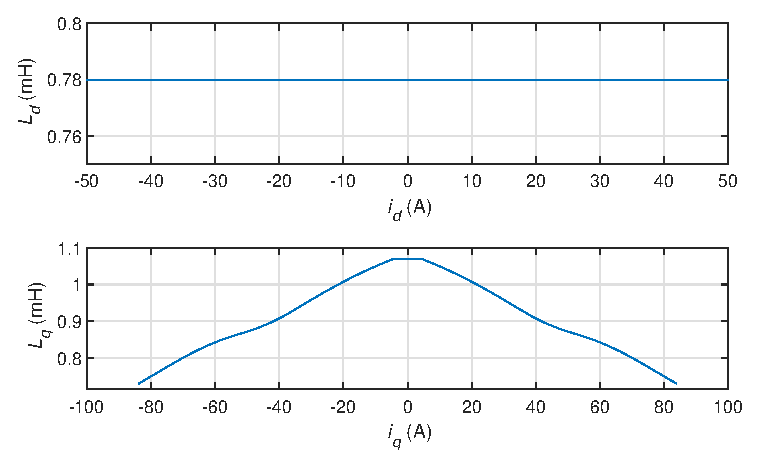
\includegraphics[width=0.7\textwidth]{Figures/ldq_manufacturer.eps}
	\caption[Manufacturer inductance curves.]{Manufacturer inductance curves.}
	\label{fig:inductance_manufacturer} %chktex 24
\end{figure}

Note that replacing the manufacturer tables with the characterized inductance curves from the appendix should not have a significant impact on the controller performance, only affecting the current references passed to the controller. The process to generate the current references and the controller structure remains the same despite the inductance curves.